\chapter{Implementation}\label{ch:implementation}

This chapter describes how the theoretical basics from \autoref{ch:methodology} interplay and how they are used in this thesis.
In this thesis, a tool is developed that offers text queries, detailed document inspection and queries for semantically or visually similar documents to the user.
\autoref{sec:offline-processing} outlines the steps carried out before the application is operative, 
\autoref{sec:ui} is about the resulting application and 
\autoref{sec:trade-off} discusses the dilemma faced when balancing memory usage and query time. 
Specific parameter choices are explained in \autoref{ch:evaluation}.


\section{Offline Processing}\label{sec:offline-processing}
This section outlines implementation details of the data fed into the database, the database itself and the baseline topic analysis approach compared to this work's application.
 % Database
\subsection{Database}\label{subsec:impl-db}
First, the content of the \databaseName{} database is described, then, the initialization, insertion and updating process of filling the database are explained 
and finally, the process of querying is outlined.

% content
\subsubsection*{Content of the database}
In this work, the database is filled once with data from a large unstructured corpus of \ac{pdf} files.
After the initialization of the database, it is used for queries. 
Therefore, the workflow is completely offline.

The index \textit{Bahamas} stores different embeddings of the information derived from the text layer and metadata of the documents.
As depicted in \autoref{fig:pdf2db}, not only textual information is stored in the database, 
but also information about the appearance of the first page of the \ac{pdf}.
The structure of the index is presented in \autoref{tbl:Elasticsearch-fields}.

\begin{table}[]
    \caption{Fields of the \databaseName{} database index \textit{Bahamas}.}
    \begin{tabular}{|
    >{\columncolor[HTML]{EFEFEF}}l |p{0.63\textwidth}|}
    \hline
    \cellcolor[HTML]{C0C0C0}\textbf{Field name} & \cellcolor[HTML]{C0C0C0}\textbf{Field description}                                     \\ \hline
    \_id                                        & Unique identifier of document \texttt{i}. The identifier is generated by the sha256 hash algorithm from hashlib using the \ac{pdf} file as input.\\ \hline
    doc2vec                                     & 55 dimensional \ac{d2v} embedding of \texttt{i}.                                                          \\ \hline
    sim\_docs\_tfidf                            & \ac{tfidf} embedding + all-zero flag of \texttt{i}. The all-zero flag is one if the \ac{tfidf} embedding consists of only zeros, zero else. If the embedding's dimensionality is greater than 2048, the encoder of a trained \ac{ae} is used to compress the embedding.\\ \hline
    google\_univ\_sent\_encoding                & 512 dimensional \ac{use} embedding of \texttt{i}.                                     \\ \hline
    huggingface\_sent\_transformer              & 384 dimensional \ac{sbert} embedding of \texttt{i}.                                  \\ \hline
    inferSent\_AE                               & \infersent{} embedding of \texttt{i}. Since the pretrained \infersent{} model embedding's dimension is 4096, the encoder of a trained \ac{ae} has to reduce the dimension to 2048.                                                    \\ \hline
    pca\_image                                  & 13-dimensional \ac{pca} version of first page image of \texttt{i}.                      \\ \hline
    pca\_optics\_cluster                        & Cluster of \texttt{i} identified by \acs{optics} on \ac{pca} version of image.            \\ \hline
    argmax\_pca\_cluster                        & Number of maximum \ac{pca} component as cluster of \texttt{i}.                            \\ \hline
    text                                        & Text of \texttt{i}.                                                                       \\ \hline
    path                                        & Path to \texttt{i}.                                                     \\ \hline
    \end{tabular}
    \label{tbl:Elasticsearch-fields}
\end{table}

\begin{figure}[!htb] % htp = hier (h), top (t), oder auf einer eigenen Seite (p).
    \centering
    \includesvg[width=1\textwidth]{images/Elasticsearch/PDFs_to_database}
    \caption[Database procedure]{\acp{pdf} to Database. 
    First, the data is preprocessed:
    The first page of a \ac{pdf} file is converted to an image and the complete text is extracted. 
    The images are stored in the database as well as the text and different embeddings of the text.
    Some values, such as the image or the \infersent{} embedding, have to be compressed to become a vector of at most 2048 dimensions.
    }
    \label{fig:pdf2db}
\end{figure}

% initialize, insert, update
\subsubsection*{Initialization, insertion and updating}
To facilitate working with and running the code the initialization of the database is split into multiple steps.
As depicted in \autoref{fig:init_db}, first the database is initialized by defining the index name and the mappings, i. e. the field names, types and sizes.
This step is carried out using the method \texttt{create}.

\begin{figure}[!htb] % htp = hier (h), top (t), oder auf einer eigenen Seite (p).
    \centering
    \includesvg[width=0.5\textwidth]{images/Elasticsearch/init_db.svg}
    \caption[Initialization and filling of the database]{Procedure of initialization and filling of the database.}
    \label{fig:init_db}
\end{figure}

Afterwards, the documents are created using the method \texttt{create}.
The initial creation of a document only defines the fields \texttt{id}, \texttt{text} and \texttt{path}.
% In order to maximise efficiency when updating the database, the \databaseName{}'s built-in functionality \texttt{bulk} is used.
% \texttt{bulk} sends chunks of multiple requests to the database.
% As displayed in \lst{lst:db_bulk}, \texttt{bulk} is called with the \databaseName{} client, 
% a function which yields requests and parameters, which define the return values.
% The structure of a function that yields requests is shown in \lst{lst:db_bulk_yield}.

% \begin{listing}[htp]
%     \begin{minted}{python3}
%         bulk(client, create_document_aux(src_paths, client), stats_only= True)
%     \end{minted}
%     \caption[Usage of \databaseName{}'s helper functionality \texttt{bulk}]
%     {Usage of \databaseName{}'s helper functionality \texttt{bulk} to send multiple requests to the database in chunks.
%     }
%     \label{lst:db_bulk}
% \end{listing}

% \begin{listing}[htp]
%     \begin{minted}{python3}
%         def create_document_aux(src_paths: list, client: Elasticsearch):  
%             for path in src_paths:           
%                 id = get_hash_file(path)
%                 if get_doc_meta_data(client, doc_id=id) is not None:
%                     continue
%                 text = pdf_to_str(path)
%                 yield { '_op_type': 'create',
%                         '_index': 'bahamas',
%                         '_id': id,
%                         "text": text,
%                         "path": path}
%     \end{minted}
%     \caption[Method that yields requests for \texttt{bulk}]
%     {Method that yields requests for \texttt{bulk}.
%     The method checks if the document is already in the database and if not, it yields a request to create the document.
%     }
%     \label{lst:db_bulk_yield}
% \end{listing}

The embeddings are added to the documents in a third step.
% To make sure that it is possible to update embeddings individually without changing other fields, 
% a method to insert the embeddings of a specific model for all documents is created.
% The documents are updated using the \texttt{update} keyword and \texttt{bulk}.
To increase the efficiency of this step, data parallelism, i. e. parallelizing the execution of a method across multiple input values, is applied.
In this work, the data to be split among multiple processes is a set of paths to documents.
The \texttt{Pool} object from the multiprocessing module is used for data parallelism.
The steps carried out are displayed in \lst{lst:db_Pool_embeddings}.
First, the absolute paths of all documents are saved in a list.
This list is divided in \texttt{num\_cpus} many sublists of similar size.
Each process works on a sublist.
The embeddings are subsequentially inserted into the database for each sublist. 

\begin{listing}[htp]
    \begin{minted}{python3}
        with Pool(processes=num_cpus) as pool:
            for model_name in model_names:
                proc_wrap = wrapper(model_name=model_name, baseDir=src_path)
                pool.map(proc_wrap, sub_lists)
    \end{minted}
    \caption[Usage of \texttt{Pool} for data parallelism]
    {Usage of \texttt{Pool} for data parallelism.
    The paths to the documents to insert are divided into sublists which are simultaneously inserted into the database.
    Since the \texttt{Pool} object does not work with a \texttt{lambda} function, 
    a class \texttt{wrapper} is created which provides the same functionality.
    }
    \label{lst:db_Pool_embeddings}
\end{listing}

The document embeddings are added to the database using the method \texttt{update} as displayed in \lst{lst:db_Pool_update}.

\begin{listing}[htp]
    \begin{minted}{python3}
        client.update(index='bahamas', id=id, body={'doc': 
            {MODELS2EMB[model_name]: embedding}})
    \end{minted}
    \caption[Update of a database entry]
    {Update of a database entry to insert a specific embedding.
    }
    \label{lst:db_Pool_update}
\end{listing}


% search
\subsubsection*{Queries}
The default analyzer is used for the full-text search since for instance configuring a maximum token length did not seem necessary or likely to improve the results.

\begin{listing}[htp]
    \begin{minted}{python3}
        results = elastic_search_client.search(
            index='bahamas', 
            size=count,
            from_=(page*count),
            query= {'match': {
                        'text': {'query':text,
                                'fuzziness': 'AUTO',}
                    }, 
                }, source_includes=SRC_INCLUDES)
    \end{minted}
    \caption[Query to an \databaseName{} database index]{Exemplary query to an \databaseName{} database index.
    The parameters \texttt{size} and \texttt{from\_} define the number of results to return and the start index of the results.
    To enable fuzzy search a value for \texttt{fuzziness} has to be set. 
    }
    \label{lst:fuzzy_query}
\end{listing}

Moreover, the fuzzy matching option is set to \texttt{AUTO}, which means in terms of keyword or text fields that the allowed Levenshtein Edit Distance, 
i. e. number of characters changed to create an exact match between two terms, to be considered a match, is correlated to the length of the term \cite{Elasticsearch-fuzziness}.
By default, terms of length up to two characters must match exactly, terms of length three to five characters must have an edit distance of one and 
terms of length six or more characters must have an edit distance of two \cite{Elasticsearch-fuzziness}.
An exemplary query, which uses fuzzy search is given in \lst{lst:fuzzy_query}.

According to \citeauthor{Elasticsearch-kNN-HNSW}, one of \ac{knn} search's use cases is semantic document retrieval, which makes it a good fit for this task.
In this work, the approximate nearest neighbours search is used, since it is faster and the results are good enough for the purpose of this work.
The similarity measure used in this work is the cosine similarity, which calculates the \texttt{\_score} of a document according to \autoref{eq:cosine-similarity-db} from \cite{Elasticsearch-kNN-similarity}, 
where \texttt{query} is the query vector and \texttt{vector} is the vector representation of the document in the database.
The other similarity measures provided by \databaseName{} are \texttt{l2\_norm} or 
so-called Euclidian distance and \texttt{dot\_product} which is the non-auto-normalized version of the \texttt{cosine} option.
Since cosine is not defined on vectors with zero magnitude, embeddings that can return all zero vector representations, such as \ac{tfidf}, 
are enhanced with an all-zero flag before inserting them into the database.

\begin{equation}
    \frac{1 + \text{cosine}(\text{query}, \text{vector})}{2}
    \label{eq:cosine-similarity-db}
\end{equation}

In this work, the only tool from the elastic stack used is \databaseName{}.
Without Kibana, the used models are saved on disk as \ac{pkl} files.
Consequently, instead of using the \ac{knn} query structure for semantic search on embeddings provided by \databaseName{}, the normal \ac{knn} search on a field that contains an embedding is used.

% Eigendocs
\section{\eigendocs{}}\label{subsec:eigendocs}

% this work
\begin{figure}[htp] % htp = hier (h), top (t), oder auf einer eigenen Seite (p).
    \centering
    \includesvg[width=1.0\textwidth]{images/eigendocs}
    \caption[\eigendocs{} procedure]{From \acp{pdf} to \eigendocs{}.
    Firstly, the first page of a document is converted to an image.
    Then, the image is preprocessed:
    It is placed on a white canvas, to ensure all images have the same dimensions.
    Moreover, it is converted to greyscale and normalized to values between zero and one.
    Afterwards, the 2d image is reshaped to a 1d array.
    Lastly, the image is compressed using \eigendocs{}.
    }
    \label{fig:eigendocs_procedure}
\end{figure}

In this work, the \eigenfaces{} approach from \autoref{subsec:eigenface} is used to compress the images of the first page of documents.
The idea is that documents not only hold textual information but also visual information, such as layout, company logo or signature.
By mapping those images on a subspace, they ought to be grouped by visual similarity.
The procedure of the \eigenfaces{} adaption \textit{\eigendocs{}} is displayed in \autoref{fig:eigendocs_procedure}.

% procedure
The documents are first read from a directory. 
Subsequently, their first page is converted to an image and saved.
When initially filling the database, these images are read from their directory.
Firstly, the maximum height and width among all images in the corpus is calculated.
These dimensions are used to create a white canvas for each image which forms the background.
Every image is placed in the upper left corner.
Hence, assuming the selection of documents used to fit the \ac{pca} model is representative, 
scaling is not necessary and thus, the portion of white pixels on the right and bottom side encodes the dimension of the former image.
However, some images are bigger than the max values from selected data and as a consequence are scaled.
Therefore, the relative size of images in the corpus is incorporated in the resulting representation of the input images.

\begin{listing}[htp]
    \begin{minted}{python3}
        C = np.ones((max_w,max_h))
        C[:doc.shape[0],:doc.shape[1]] = rgb2gray(doc)
        documents.append(C.ravel())
    \end{minted}
    \caption{Preprocessing of the input images from \thesissupervisor{}.
    The background is a white canvas.
    The images are converted to one-dimensional greyscale values.}
    \label{lst:preproc_images}
\end{listing}

Afterwards, they are converted to greyscale images using \lst{lst:rgb2grey}.
Before returning the image, the two-dimensional image vectors are converted to one-dimensional ones as displayed in the last line of \lst{lst:preproc_images}.
The decomposition is transformed using \ac{pca} as displayed in \lst{lst:pca_svd}.
The implementation of \ac{pca} from \href{https://scikit-learn.org/stable/modules/generated/sklearn.decomposition.PCA.html}{sklearn} 
intrinsically normalizes the data as described in \autoref{subsec:eigenface} and thus, does not require the user to manually preprocess the data.


\begin{listing}[htp]
    \begin{minted}{python3}
        0.299*img[:,:,0] + 0.587*img[:,:,1] + 0.114*img[:,:,2]
    \end{minted}
    \caption{Conversion of RGB pixel values to greyscale from a script by \thesissupervisor{}.}
    \label{lst:rgb2grey}
\end{listing}

\begin{listing}[htp]
    \begin{minted}{python3}
        pca = decomposition.PCA(n_components=n_components, whiten=True, 
            svd_solver="randomized")
    \end{minted}
    \caption{Initialization of the \ac{pca} instace used to compress the image data.
    Since the \eigenfaces{} approach uses a svd\_solver, the adaption \eigendocs{} has to be implemented likewise.
    }
    \label{lst:pca_svd}
\end{listing}




% Embeddings
\subsection{Embeddings}\label{subsec:impl-embeddings}
The models used to encode the textual data from the data corpus are outlined below with regard to implementation details.

\subsubsection*{\ac{tfidf}}\label{subsubsec:impl-tfidf}

% overall architecture
The \ac{tfidf} model has to be initialized and trained on the data corpus to build a data-specific vocabulary.
An exemplary implementation is given in \lst{lst:impl-tfidf}.
The \texttt{TfidfVectorizer} is provided by the \texttt{scikit-learn} package.
When initializing the model, the parameters define not only the input type but also the way the data is preprocessed.
The \texttt{input} parameter defines the input type, i.e.\ \texttt{content} means that the input is a list of strings or bytes, 
whereas \texttt{file} assumes the input has a \texttt{read} method and \texttt{filename} denotes a list of filenames as input \cite{tfidf-scikit-learn}.
An embedding is obtained using the command from \lst{lst:encode-tfidf}.

\begin{listing}[htp]
    \begin{minted}{python3}
        tfidf_model = TfidfVectorizer(input='content', 
                    preprocessor=TfidfTextPreprocessor().transform, min_df=3, 
                    max_df=int(len(docs)*0.07))
        tfidf_model.fit(documents)
    \end{minted}
    \caption[Initialization of the \ac{tfidf} model]{Initialization of the \ac{tfidf} model.
    Firstly, an instance of the \texttt{TfidfVectorizer} class is created.
    Secondly, the \texttt{fit} method is called to fit the model on the documents.
    }
    \label{lst:impl-tfidf}
\end{listing}

\begin{listing}[htp]
    \begin{minted}{python3}
        tfidf_model.transform(text).todense()
    \end{minted}
    \caption[Encoding a text using the \ac{tfidf} model]{Encoding a text using the \ac{tfidf} model.
    }
    \label{lst:encode-tfidf}
\end{listing}

The \texttt{preprocessor} parameter defines the preprocessing, i.e.\ string transformation, stage.
It is possible to override the default with a custom preprocessing function.
The parameters \texttt{min\_df} and \texttt{max\_df} define the minimum and maximum document frequency of a word in the corpus to be considered relevant.
The default values are $1$, i.e.\ a term has to appear at least once, and $1.0$, i.e.\ a term appears at most in all documents, respectively \cite{tfidf-scikit-learn}.

By default, the \texttt{scikit-learn} implementation uses the \texttt{norm='l2'} parameter, i.e.\ the Euclidean norm \cite{tfidf-scikit-learn}.
The implementation of \ac{tfidf} in \texttt{scikit-learn} is different from the original \ac{tfidf} definition.
The difference is the calculation of the \ac{idf} part, which is given in \autoref{eq:tfidf-scikit-learn} from \cite{tfidf-scikit-learn}.
The one is added to $M_{ij}$ due to the parameter \texttt{smooth\_id=True} by default to prevent zero divisions \cite{tfidf-scikit-learn}
and to avoid logarithmic divergences due to a zero argument \cite{glove2014}.
After calculating the \ac{tfidf} values, they are normalized by the Euclidean norm 
$v_{norm} = \frac{v}{\left\| v \right\|_{2}} = \frac{v}{\sqrt{v_1^{2} + v_2^{2} + ... + v_M^{2}}}$.

\begin{equation}
    \text{idf}(w_{ij}) = \log \frac{1 + M}{1 + M_{ij}} + 1    
    \label{eq:tfidf-scikit-learn}
\end{equation}

% pipeline
In this work, the text of the PDFs is first extracted, then preprocessed using a custom preprocessor and afterwards embedded using the \texttt{TfidfVectorizer}.
The \ac{tfidf} weights are the embedding.
Before storing the \ac{tfidf} weights in the database, they are enhanced with an all-zero flag.
The all-zero flag ensures that no all-zero vectors are stored in the database by extending those that have a zero magnitude with a "1" entry and "0" otherwise.
All-zero \ac{tfidf} weights indicate that a document does not have any terms with the vocabulary in common.
Since the vocabulary is kept relatively small with respect to the number of different words in the data corpus to reduce the dimensionality of the embeddings, 
it is not unlikely that a document does not contain any of the vocabulary terms.
The all-zero flag is necessary because the cosine similarity used to query for similar documents in the database cannot handle vectors of zero magnitude.
This alteration does not change the cosine similarity between non-zero magnitude vectors, 
since the additional zero adds no supplementary information to the calculation of the cosine similarity.
The vectors with a one in the all-zero flag column have a cosine similarity of one.
The pipeline in \autoref{fig:tfidf_embedding} visualizes these steps.

\begin{figure}[!htb] % htp = hier (h), top (t), oder auf einer eigenen Seite (p).
    \centering
    \includesvg[width=1\textwidth]{images/embeddings/tfidf/TFIDF_embedding.svg}
    \caption[\acs*{tfidf} pipeline]{\acs*{tfidf} pipeline.
    Firstly, the text extracted from the documents is preprocessed using a custom preprocessor.
    Then, the \acs*{tfidf} values are obtained from the \texttt{TfidfVectorizer}.
    Afterwards, the all-zero flag is added to the \acs*{tfidf} weights.
    If the resulting dimensionality is bigger than 2048, the encoder of an \acs*{ae} is used to reduce the dimensionality.
    The results are stored in the database.
    }
    \label{fig:tfidf_embedding}
\end{figure}


\begin{figure}[!htb] % htp = hier (h), top (t), oder auf einer eigenen Seite (p).
    \centering
    \includesvg[width=1\textwidth]{images/embeddings/tfidf/TFIDF_preprocessing.svg}
    \caption[Preprocessing]{Preprocessing visualized using an example text.
    The stop word removal implicitly tokenizes the text.}
    \label{fig:preprocessing}
\end{figure}

% custom preprocessing
In this work, a custom preprocessing function is used.
The preprocessing steps are visualized in \autoref{fig:preprocessing}.
Firstly, the accents are stripped from the text.
Then, all new line symbols are replaced with a whitespace.
Afterwards, the text is converted to lowercase.
Then the numbers are discretized, i.e.\ all numbers between 0 and 99999 are replaced with the string \texttt{SMALLNUMBER}, 
numbers bigger than 99999 are replaced with the string \texttt{BIGNUMBER} and floats are replaced with the string \texttt{FLOAT}.
The next step is to remove all punctuation symbols.
To ensure empty tokens generated by prior preprocessing steps are omitted, 
all sequences of multiple subsequent whitespaces are discarded.
After that, the symbols for numbers are enclosed with pointed brackets, e.g. \texttt{<SMALLNUMBER>}.
Then, the text is tokenized, i.e.\ split at whitespaces, and stop words are omitted.
The stop word list is provided by the \texttt{nltk} package 
and consists of common English stop words.
Afterwards, the tokens are lemmatized.
The lemmatizer used is \texttt{WordNetLemmatizer} from the \texttt{nltk} package.
\texttt{WordNetLemmatizer} uses the English lexical database \texttt{WordNet} to return valid stems \cite{nltk-lemma-wordnet}
In the end, the tokens are joined to a string and returned.

% Autoencoder
Since the dimensionality of the \ac{tfidf} embeddings is big for a large text corpus, 
an \ac{ae} is used to reduce the dimensionality of the embedding if its dimensionality exceeds 2048.

\subsubsection*{\ac{d2v}}\label{subsubsec:impl-doc2vec}

The library \texttt{gensim} provides the \ac{d2v} model used in this work.
The model is initialized with input data of type \texttt{tagged documents}, which are documents with (numerical) tags.
In this work, the default parameters are used.
%The parameter \texttt{dm} determines the training algorithm used.
%The value \texttt{dm=1} specifies the \ac{pvdm} algorithm, while \texttt{dm=0} specifies the \ac{pvdbow} algorithm \cite{gensim-doc2vec}.
The default algorithm is \ac{pvdm} \cite{gensim-word2vec-init}.
The parameters \texttt{vector\_size} and \texttt{window} define the dimensionality of the embeddings and the size of the window, 
i.e.\ the maximum distance between the current and the predicted word, respectively.
The default value for \texttt{vector\_size} is 100, whereas the default window size is 8 \cite{gensim-word2vec-init, gensim-doc2vec-init}.
The \texttt{min\_count} parameter defines a threshold below which words will be ignored.
Its default value is 5.
The \texttt{workers} parameter denotes the number of threads to be used for training.
The default value is 1 \cite{gensim-word2vec-init}.
The \texttt{epochs} parameter specifies the number of iterations over the corpus.
The default value is 10.
By default, the hierarchical softmax algorithm, i.e.\ \texttt{hs=1}, is used for training \cite{gensim-doc2vec}.
Many \ac{d2v} default values are adopted from \ac{w2v} since the \texttt{gensim} \ac{d2v} implementation inherits from the \ac{w2v} implementation.


\subsubsection*{\infersent{}}\label{subsubsec:impl-infersent}

% parameters
The \infersent{} model is implemented using PyTorch \cite{HfsentTrans2019}.
The parameters used to initialize the model are presented in \lst{lst:infersent-params}.
The parameter \texttt{version} in line \ref{line:infersent_version} indicates whether 
the model is trained with \acs{glove} or fastText for the value 1 or 2 respectively.
Since the model is precomputed, it is not possible to change certain parameters, 
such as the word embedding dimension \texttt{word\_emb\_dim} or the dimension of the output vectors \texttt{enc\_lstm\_dim}.

\begin{listing}[htp]
    \begin{minted}[escapeinside=||]{python3}
        'bsize': 64, 
        'word_emb_dim': 300, 
        'enc_lstm_dim': 2048,  
        'pool_type': 'max', 
        'dpout_model': 0.0, 
        'version': 1|\phantomsection\label{line:infersent_version}|
    \end{minted}
    \caption{Parameters of the \infersent{} model.
    }
    \label{lst:infersent-params}
\end{listing}

% state dict
The steps necessary to create a working instance of the \infersent{} model are presented in \lst{lst:infersent-init}.
After the \infersent{} model is initialized in line \ref{line:init}, the \texttt{state\_dict} of the model is loaded in line \ref{line:state_dict}.
This dictionary consists of learnable parameters, i.e.\ weights and bias, of the model.
The \texttt{state\_dict} is obtained from the \ac{pkl} file of \infersent{} as stated in \cite{download-infersent}.
The path to the word embeddings is set in line \ref{line:w2v_path}.
Finally, in line \ref{line:vocab}, the vocabulary of the model is built. 
More precisely, only those embeddings needed are kept while the rest is discarded.

\begin{listing}[htp]
    \begin{minted}[escapeinside=||]{python3}
        infersent = InferSent(params_model)|\phantomsection\label{line:init}|
        infersent.load_state_dict(torch.load(model_path))|\phantomsection\label{line:state_dict}|
        infersent.set_w2v_path(w2v_path)|\phantomsection\label{line:w2v_path}|
        infersent.build_vocab(docs, tokenize=True)|\phantomsection\label{line:vocab}|
    \end{minted}
    \caption{Initializing the \infersent{} model.
    }
    \label{lst:infersent-init}
\end{listing}

% GloVe
% Initially, in this work, the \infersent{} model was based on \acs{glove} word embeddings.
% \acs{glove} is a global log-bilinear regression model for unsupervised learning of vector representations of words \cite{glove2014}. 
% According to \citeauthor{glove2014}, the model captures global corpus statistics directly.
% %The complexity of the model is bound by $O(V^2)$, $V$ being the vocabulary size.
% %However, \citeauthor{glove2014} claim it is better than the worst case stated above and rather in $O(C)$, $C$ being the corpus size.
% The \acs{glove} model is trained on ratios of co-occurrence probabilities of words from the corpus, 
% which correlate with the relationship between the words. % \cite{glove2014}.
% \citeauthor{glove2014} introduce rules for a weighting function to ensure neither rare nor frequent co-occurrences are overweighted.
% It is possible to download embeddings computed by \acs{glove}, instead of using the algorithm to generate them.
% The precomputed word embeddings are stored in a 5.65 \ac{gb} text file.
% The file contains 840 B tokens and a vocabulary of 2.2 M cased 300-dimensional vector representations of words \cite{download-glove}.
% According to \citeauthor{UniversalSentEnc2018}, \acs{glove} introduces bias in terms of ageism, racism and sexism into the model.

% own W2V
In this work, a custom set of vector representations of words is used.
The custom word embeddings are computed by a \ac{w2v} model trained on 2048 randomly selected documents from the Bahamas dataset 
which reduces the run time of the script.
The only parameter which differs from the default settings of \ac{w2v} is the \texttt{vector\_size} which is set to 300.
After the \ac{w2v} model is trained, the word embeddings are saved in a file 
whose file path is the value of \texttt{w2v\_path} in line \ref{line:w2v_path} of \lst{lst:infersent-params}.
% The file is post-processed to be compatible with the \infersent{} model.
% To be more precise, only lines that consist of at least two whitespace-separated char sequences are kept.
% Usually, word embeddings stored in a text file are structured in a way that 
% the first char sequence is the word and the following numbers are the vector representation of the word.

% Autoencoder
In this work, an \ac{ae} is used to reduce the dimensionality of the \infersent{} embedding.


\subsubsection*{\ac{use}}\label{subsubsec:impl-use}

The \ac{use} model implemented with TensorFlow \cite{HfsentTrans2019}.
In this work, the fourth version of the model is used.
The implementation from Tfhub uses the \ac{dan} architecture \cite{UniversalSentEnc-dev}.
The file is about 1 \ac{gb}. % and thus, loading the model takes a while.
It is not necessary to preprocess the data for the model \cite{UniversalSentEnc-dev}.

\section{\ac{sbert}}\label{sec:impl-sbert}

The \ac{sbert} model is provided by PyTorch \cite{HfsentTrans2019}.
An instance of the model is obtained by initializing it as shown in \lst{lst:impl-sbert}.
The model consists of a \ac{bert} transformer, which has a \texttt{max\_seq\_length} of $128$. 
It does not convert inputs to lowercase by default \cite{sbert-dev}.
The output of the transformer is passed to a pooling layer, which is initialized with the \texttt{pooling\_mode} parameter.
The default is \texttt{mean\_pooling}, which calculates the mean of the output vectors of the transformer.
The other options are \texttt{cls\_token\_pooling}, which returns the output of the first token, 
\texttt{max\_pooling}, which returns the maximum value of the output vectors,
and \texttt{pooling\_mode\_mean\_sqrt\_len\_tokens}.
The word embedding dimension is 384 by default \cite{sbert-dev}.

\begin{listing}[htp]
    \begin{minted}{python3}
        SentenceTransformer('paraphrase-MiniLM-L6-v2')
    \end{minted}
    \caption[Initialization of the \ac{sbert} model]{Initialization of the \ac{sbert} model.
    }
    \label{lst:impl-sbert}
\end{listing}

\subsubsection*{\acl{ae}}\label{subsubsec:impl-autoencoder}

In this work, an \ac{ae} is used to reduce the dimensionality of the \infersent{} and the \ac{tfidf} embeddings.
Since the \infersent{} model is pretrained, it is not possible to change the dimensionality of the embedding without a considerably big effort,
i.e.\ retraining the model on a sufficiently large data corpus and reconfiguring the model's parameters.
Therefore, it is not feasible to change the dimensionality of the \infersent{} embedding, but rather add a supplementary layer after the model 
to produce the final embedding.
Similarly, the \ac{tfidf} embedding dimension correlates with the vocabulary size and thus, the size of the data corpus.
Further reducing the vocabulary size would decrease the \ac{tfidf} model's quality.
Hence, the idea is to use the encoder of an \ac{ae} to reduce the dimensionality of the \infersent{} and the \ac{tfidf} embedding.

\begin{figure}[!htb] % htp = hier (h), top (t), oder auf einer eigenen Seite (p).
    \centering
    \includesvg[width=1.0\textwidth]{images/embeddings/autoencoder/autoencoder-impl.svg}
    \caption[Architecture of the \acs*{ae}]{Architecture of the \acs*{ae}.}
    \label{fig:impl-ae}
\end{figure}

The implementation was provided by the blog post from \cite{impl-src-ae}.
It uses the library keras\footnote{https://keras.io/ (last accessed: 19/11/2023)}.
The architecture is adapted to fulfil the needs of the specific context.
It is presented in \autoref{fig:impl-ae}.

% Clustering
\subsection{Clustering using \acs*{optics}}\label{subsec:impl-optics}

\begin{figure}[!htb] % htp = hier (h), top (t), oder auf einer eigenen Seite (p).
    \centering
    \includesvg[width=1\textwidth]{images/OPTICS/OPTICS_procedure.svg}
    \caption[\ac{optics} procedure]{The first page of each document is converted to an image.
    The image is preprocessed, i.e. conversion to greyscale and resizing.
    }
    \label{fig:OPTICS_procedure}
\end{figure}

Similar to the approach from \citeauthor{OPTICS1999}, \ac{optics} is used to cluster the images of the first page of documents in this work.
The procedure is displayed in \autoref{fig:OPTICS_procedure}.
There were two different preprocessing approaches:
\begin{enumerate}
    \item \label{pt:32}The images were first preprocessed to 32x32 normalized greyscale pixels (cf. \cite{OPTICS1999}) as visualized in \autoref{fig:preprocessed_docs_32x32}
    and afterwards compressed to 13-dimensional vectors using \ac{pca}.
    \item \label{pt:eigendocs}The technique \eigendocs{} from \autoref{subsec:eigenface} 
    was used to compress the images to 13-dimensional normalized greyscale images as displayed in \autoref{fig:preprocessed_docs_eigendocs}.
\end{enumerate}


% preprocessed images
\begin{figure}[!htb] % htp = hier (h), top (t), oder auf einer eigenen Seite (p).
    \centering
    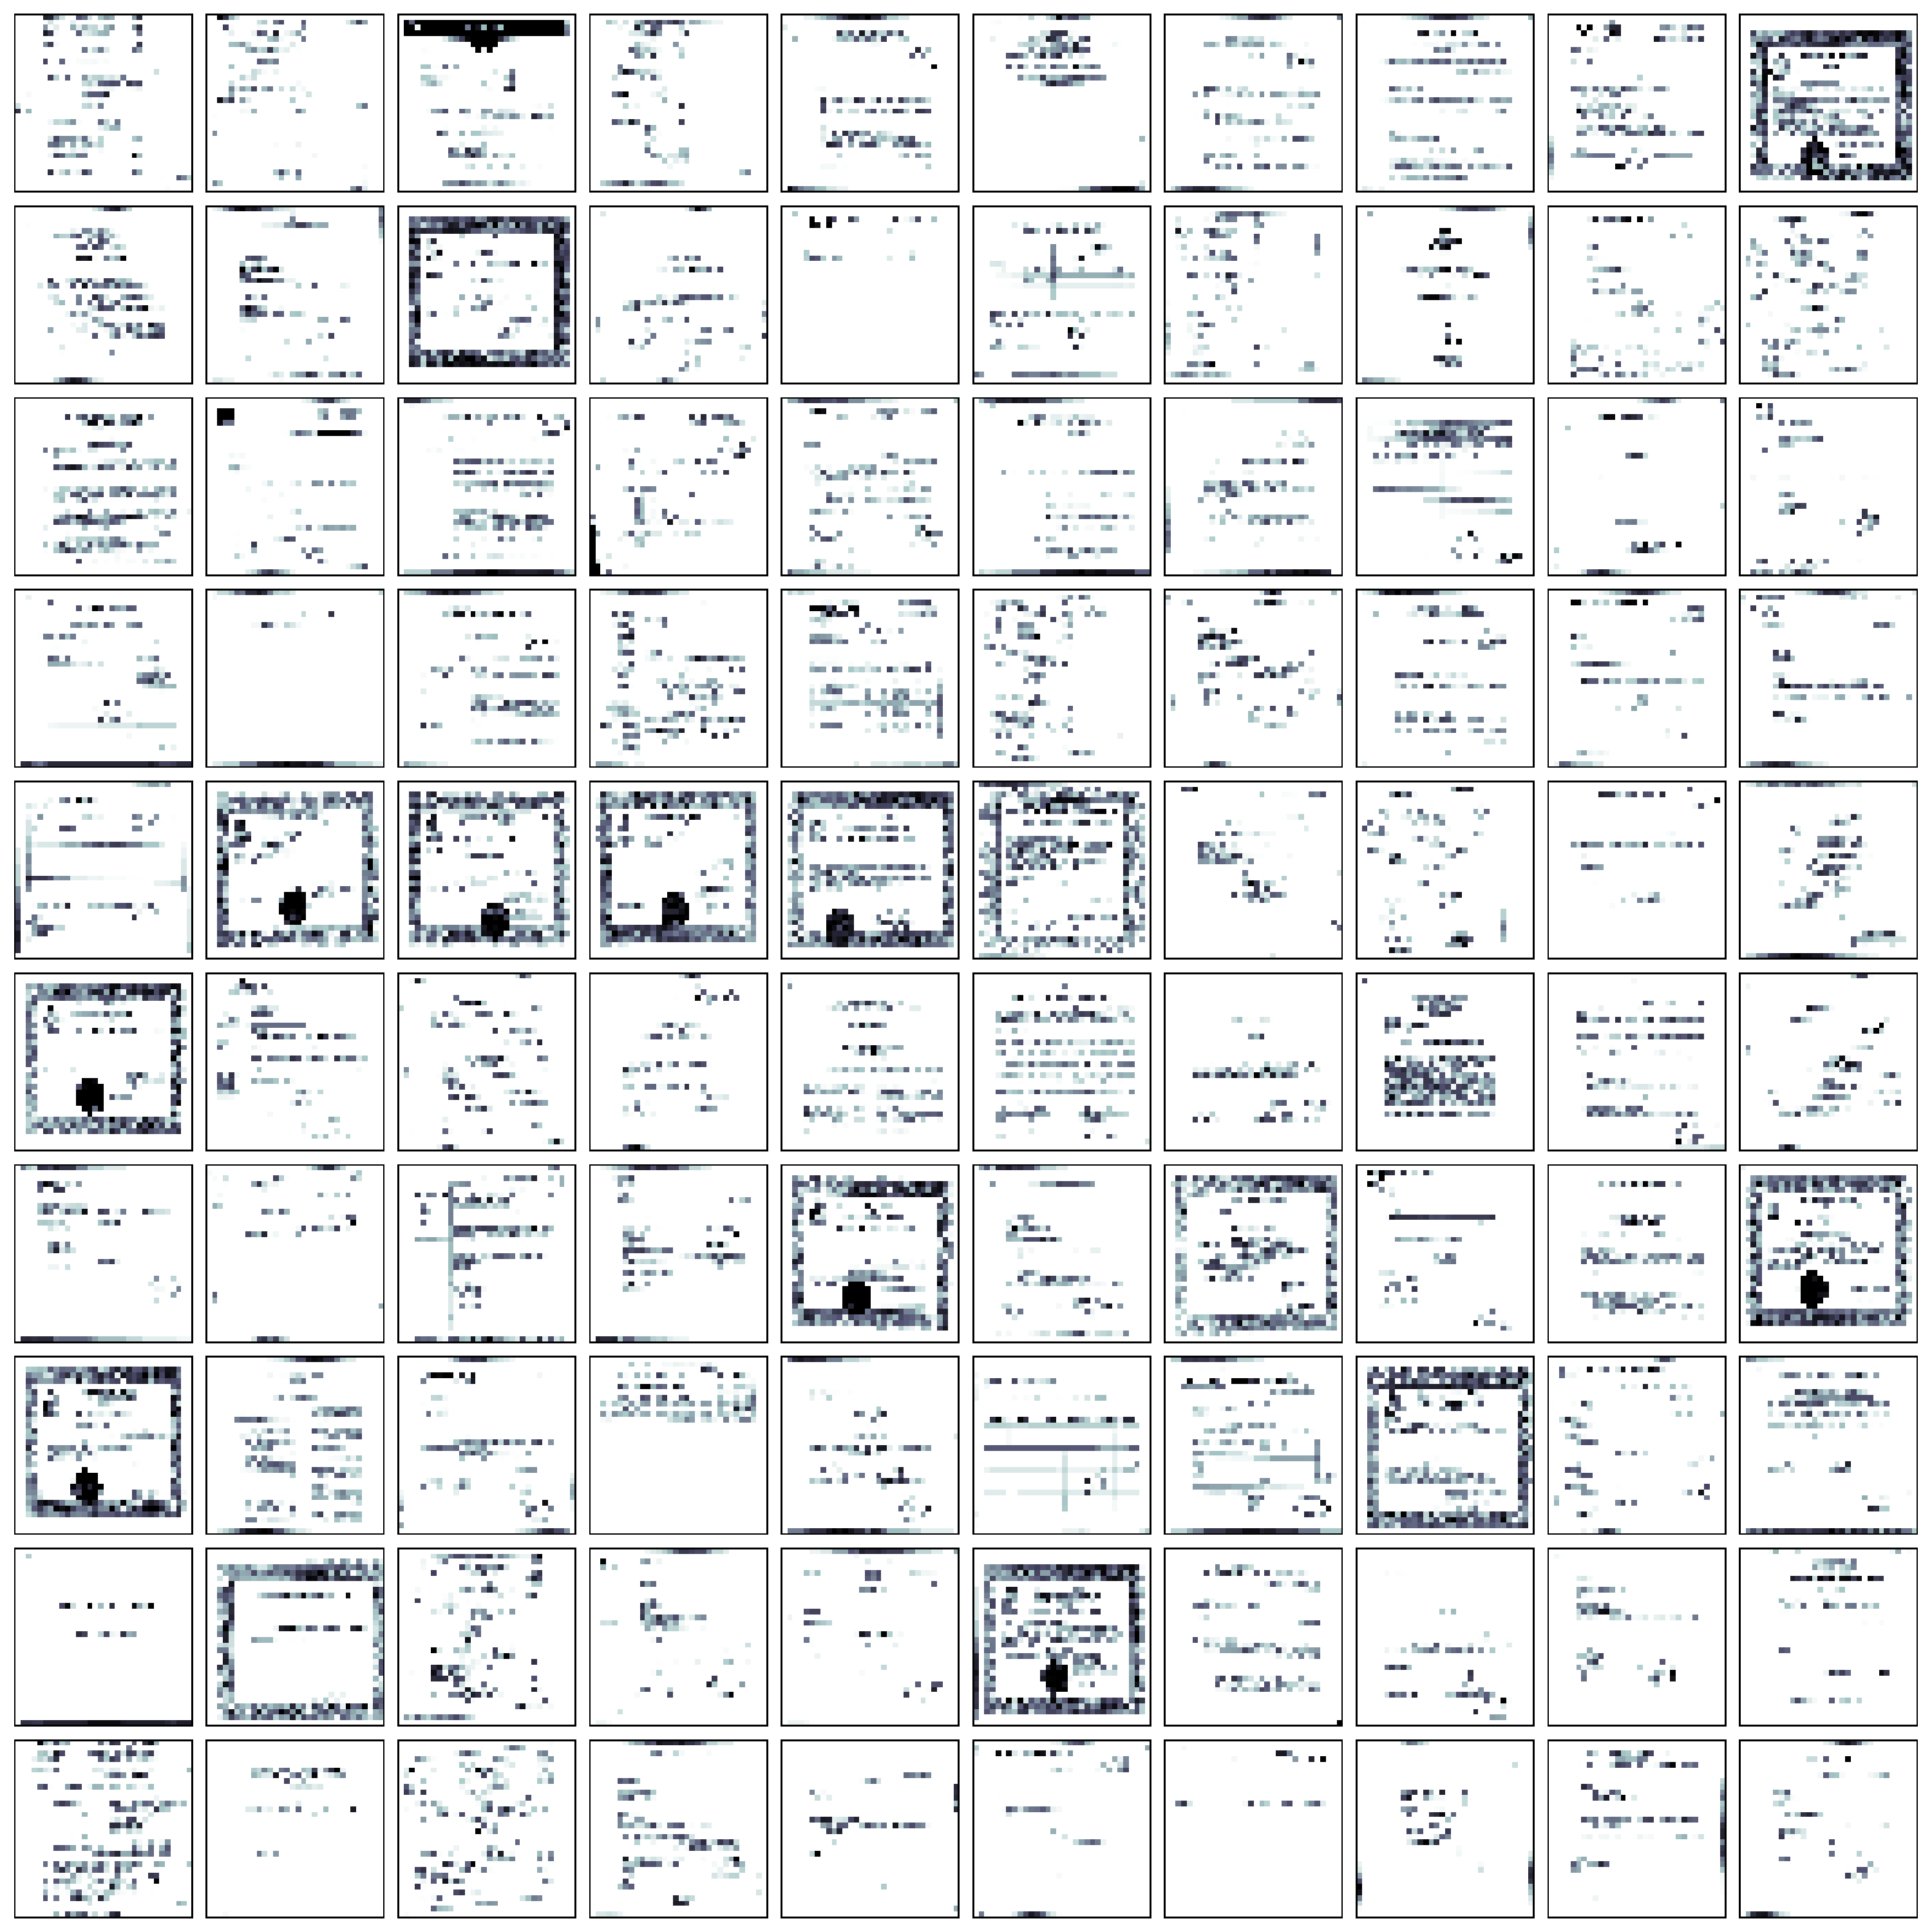
\includegraphics[width=1\textwidth]{images/OPTICS/32x32/preprocessed_docs.pdf}
    \caption[Preprocessing to 32x32 normalized greyscale pixels]{Preprocessing of 100 documents to 32x32 normalized greyscale pixels.
    }
    \label{fig:preprocessed_docs_32x32}
\end{figure}


\begin{figure}[!htb] % htp = hier (h), top (t), oder auf einer eigenen Seite (p).
    \centering
    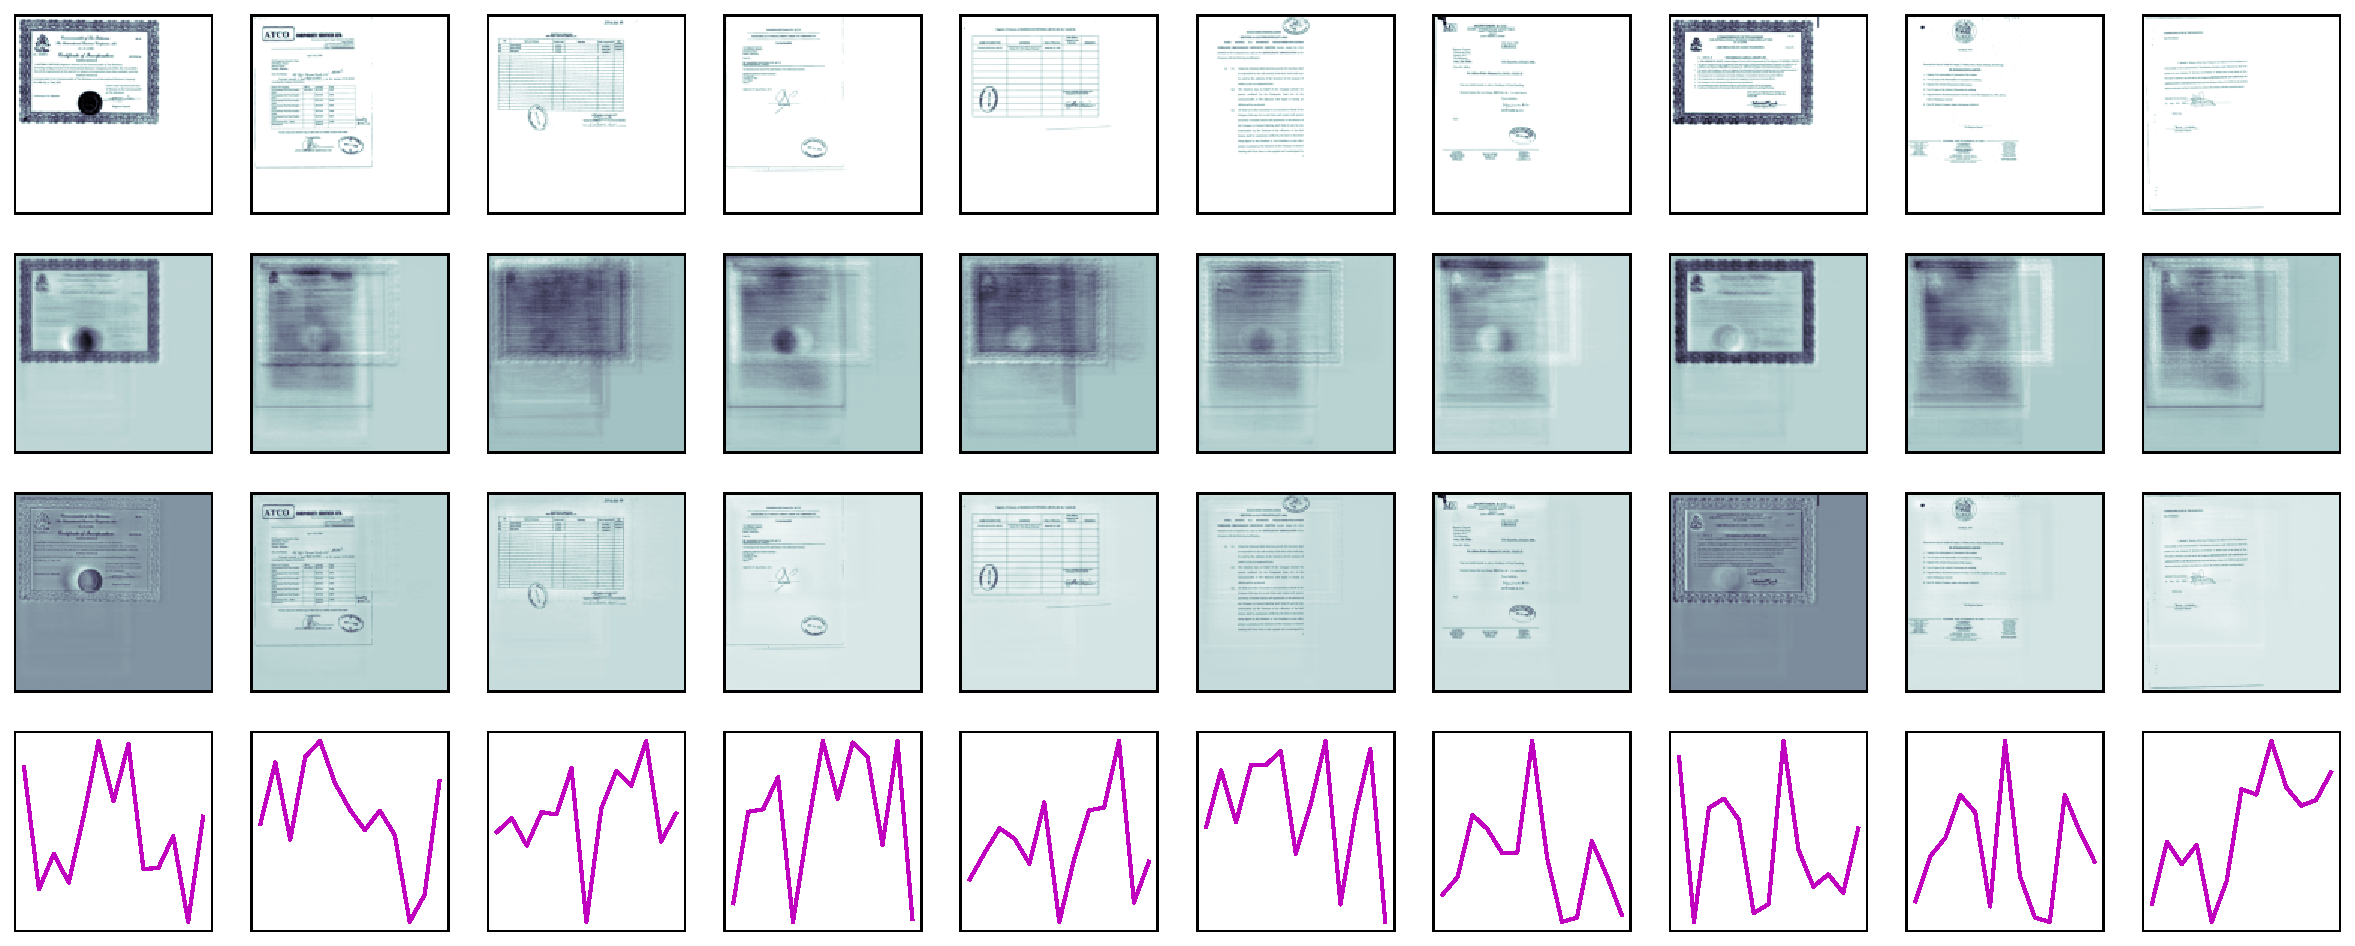
\includegraphics[width=1\textwidth]{images/Eigendocs/transformation/eigendocs.pdf}
    \caption[Preprocessing 10 randomly selected documents from the test set]{10 randomly selected documents from the test set.
    The number of images in the test set is 561, while the \ac{pca} model was fit to 1680 training images.
    The original images are displayed in the first row.
    The second row shows the reconstruction from their compressed version in the fourth row.
    The third row shows the reconstruction error, i.e. the difference between the reconstructed and the original image.
    The last row presents the greyscale values of the compressed 13-dimensional image as a line.
    }
    \label{fig:preprocessed_docs_eigendocs}
\end{figure}

The reachability distance ordered by \ac{optics} is displayed in \autoref{fig:reachability_plots}.
%The resulting clusters are displayed in \autoref{fig:optics_cluster}.

% reachability plot
\begin{figure}%
    \centering
    \subfloat[\centering The reachability plot of the documents preprocessed according to \autoref{pt:32} (cf. \cite{OPTICS1999}).]{{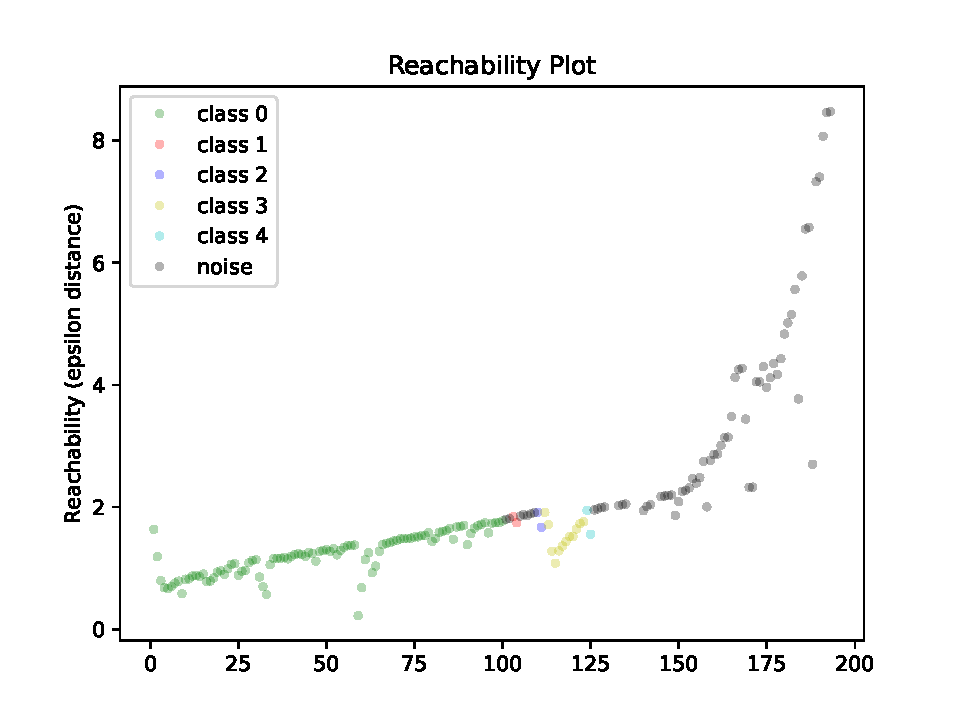
\includegraphics[width=5cm]{images/OPTICS/32x32/reachability_plot_32x32_pca_13dim.pdf} }}%
    \qquad
    \subfloat[\centering The reachability plot of the documents preprocessed according to \autoref{pt:eigendocs} (i.e. \eigendocs{}).]{{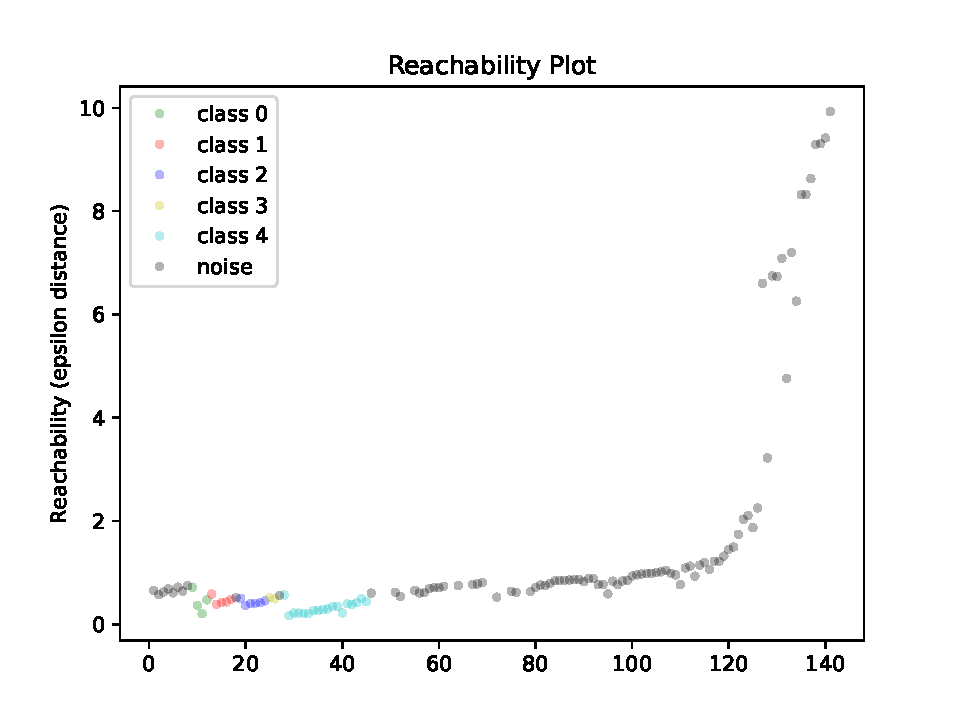
\includegraphics[width=5cm]{images/OPTICS/eigendocs/reachability_plot_13dim_eigendocs.pdf} }}%
    \caption[Reachability distances]{The plot was created using the \ac{optics} algorithm from the Python library scikit-learn.
    It shows the reachability distance of each document to its predecessor in the order list.}%
    \label{fig:reachability_plots}%
\end{figure}

% code
The configurations used when initializing an \ac{optics} model greatly influence the clusters returned.
The parameter \texttt{max\_eps} is infinity by default but can be specified by the user to reduce complexity and runtime.
According to literature, \texttt{max\_eps} should be big enough to include almost all points in a cluster.
The way the reachability plot is used to extract clusters is dependent on the \texttt{cluster\_method}. 
One can choose either \texttt{dbscan} or \texttt{xi} as a clustering method.
The parameters \texttt{min\_samples} and \texttt{eps} influence the cluster sizes and number of clusters found for a given clustering approach.
The value of \texttt{eps} defines the distance between two points to still be considered neighbours 
and can be chosen by consulting the reachability plot.
The code to initialize an exemplary \ac{optics} model is displayed in \lst{lst:optics_model}.

\begin{listing}[htp]
    \begin{minted}{python3}
        optics_model = OPTICS(cluster_method='dbscan', min_samples=2, max_eps=10, 
            eps=0.5)
    \end{minted}
    \caption[Initialization of the \ac{optics} model]{Initialization of the \ac{optics} model.
    The minimum number of samples \texttt{min\_samples} in a cluster corresponds to \textit{minPts}.
    }
    \label{lst:optics_model}
\end{listing}


% topic analysis
\subsection{Topic analysis}\label{impl-topic-modeling}

Two topic analysis approaches are outlined below.
The first one serves as the baseline model of this thesis and 
the second one is used multiple times throughout the application to visualize results obtained by queries.


\subsubsection*{\ac{t2v}}\label{subsubsec:impl-top2vec}

\citeauthor{Top2Vec2020}'s \ac{t2v} model is provided in the Python library \ac{t2v} \cite{Top2Vec2020}.
The non-changeable default values and settings of the model are listed below.
The word and document embeddings are generated by the \ac{d2v} version \ac{pvdbow}.
It has a window size of 15, uses hierarchical softmax, a minimum count of 50, a vector size of 300 and a sub-sampling threshold of $10^5$.
% dimensionality reduction
\ac{umap}'s hyperparameters are set to 15 nearest neighbours, cosine similarity as the distance metric and 5 as the embedding dimension in \citeauthor{Top2Vec2020}'s work.

In this work, a class is implemented, which uses the \ac{t2v} library.
When initiating an instance of this class, the \ac{t2v} model is trained on the given document corpus as displayed in \lst{lst:init-top2vec}.
The class provides methods to query for the number of topics as well as the 
most similar topics and documents to an input keyword.
The most similar topics can be visualized using \wordcloud{}s.
The core functionalities are implemented by the \ac{t2v} library, but the class is used to modify the return values to be compatible with the \ac{ui}.


\begin{listing}[htp]
    \begin{minted}{python3}
        Top2Vec(documents=self.documents, speed='fast-learn', workers=8)
    \end{minted}
    \caption[Initialization of the \ac{t2v} model]
    {Initialization of the \ac{t2v} model.
    }
    \label{lst:init-top2vec}
\end{listing}

\section{\wordcloud{}}\label{sec:impl-wordcloud}

The implementation of \wordcloud{}s in this thesis is based on the Python library \textit{wordcloud} \cite{wordcloud-dev}.
This implementation removes English stop words from the text by default.
The input text is split into tokens using a regex.
By default, plurals are removed if their singular version is present and their frequency is added to their singular version.
By default, numbers are not included as tokens.

% custom preprocessing
In order to ensure that the words presented are interpretable, the input text is preprocessed.
A lemmatizer is used to ensure stemmed words exist.
The lemmatizer used is \texttt{WordNetLemmatizer} from the \texttt{nltk} package as displayed in \lst{lst:impl-preproc-wordcloud}.

% initialization
The \wordcloud{} is initialized as shown in \lst{lst:impl-wordcloud}.

\begin{listing}[htp]
    \begin{minted}{python3}
        lemmatizer = WordNetLemmatizer()
        tokens = [lemmatizer.lemmatize(token) for token in tokens]
    \end{minted}
    \caption[Custom preprocessing of \wordcloud{} input]
    {Custom preprocessing of \wordcloud{} input.
    }
    \label{lst:impl-preproc-wordcloud}
\end{listing}

\begin{listing}[htp]
    \begin{minted}{python3}
        wordcloud = WordCloud(width=800, height=500, random_state=21, 
            contour_width=3, max_font_size=110, background_color='white', 
            max_words=5000).generate(','.join(tokens))
    \end{minted}
    \caption[Initialization of the \wordcloud{}]
    {Initialization of the \wordcloud{}.
    }
    \label{lst:impl-wordcloud}
\end{listing}



% Slurm/ Server

\subsection{\slurm{}}\label{subsec:slurm}

Since the data corpus is too big to be processed locally on a \localMaschineStats{}, the Chair \ac{ies} has offered to provide computational means to solve this problem.
The scripts can be processed by multiple nodes which are managed by \slurm{}.

\slurm{} is an open-source management tool for Linux clusters \cite{slurm-online}.
It allocates resources, i.e.\ compute nodes, and provides the means to start, execute and monitor jobs \cite{slurm-online, slurm2003}.

The so-called \slurm{} daemons control nodes, partitions, jobs and job steps \cite{slurm-online}.
A partition is a group of nodes and a job is the allocation of resources, i.e.\ compute nodes, to a user for a limited period of time.
A basic visualization of the architecture is given in \autoref{fig:slurm-architecture}.

\begin{figure}[!htb] % htp = hier (h), top (t), oder auf einer eigenen Seite (p).
    \centering
    \includesvg[width=0.7\textwidth]{images/slurm/slurm_architecture}
    \caption[\slurm{} architecture]{\slurm{} architecture. The management node has a \texttt{slurmctld} daemon, while every compute node has a \texttt{slurmd} daemon.
    The nodes communicate.
    The user can use certain commands, for instance \texttt{srun} and \texttt{squeue}, anywhere on the cluster.
    }
    \label{fig:slurm-architecture}
\end{figure}

% sbatch scripts
A job is started by a \texttt{sbatch} script.
This script defines the \texttt{partition}, the \texttt{job-name}, the number of \texttt{nodes}, the \texttt{cpus-per-task}, the memory \texttt{mem} allocated, 
the \texttt{time} limit and the path to store \texttt{error} and \texttt{output} logs.
It is possible to work on multiple \acp{cpu} simultaneously to divide the workload of a task.
In this work, multiple \texttt{sbatch} scripts are used to carry out a variety of tasks.
A summary of the tasks and scripts is given in \autoref{tbl:sbatch-scripts}.


\begin{table}[]
    \caption{A selection of \texttt{sbatch} scripts used in this work.}
    \begin{tabular}{|
    >{\columncolor[HTML]{EFEFEF}}p{0.28\textwidth} |p{0.68\textwidth}|}
    \hline
    \cellcolor[HTML]{C0C0C0}\textbf{Name of sbatch script} & \cellcolor[HTML]{C0C0C0}\textbf{Description}                                                                                                                                                                                                                      \\ \hline
    ae\_config.sh                                          & Comparison of different \ac{ae} architectures in terms of the metrics cosine similarity and \ac{rsme}.                                                                                                                                                                     \\ \hline
    allocate\_res.sh                                       & Allocates resources to enable a \ac{ssh} tunnel connection from a local \ac{vscode} instance to the server of the \ac{ies}. 
                                                                When enabled, the database content can be displayed with the \databaseName{} plugin.\\ \hline
    create\_database.sh                                    & Initializes the database by specifying fields.                                                                                                                                                                                                                    \\ \hline
    create\_documents.sh                                   & Inserts the document's metadata information, i.e.\ path and text.                                                                                                                                                                                                   \\ \hline
    elasticContainer.sh                                    & Starts the \databaseName{} container using the headless \texttt{podman-compose up} command.                                                                                                                                     \\ \hline
    init\_database.sh                                      & Initializes database, subsequentially inserts documents metadata, embeddings and clusters.                                                                                                                                                                        \\ \hline
    insert\_clusters.sh                                    & Inserts \ac{pca} weights, \ac{optics} and argmax clusters.                                                                                                                                                                      \\ \hline
    insert\_embeddings.sh                                  & Subsequentially inserts embeddings of documents.                                                                                                                                                                                                                  \\ \hline
    own\_w2v\_model.sh                                     & Creates and saves custom \ac{w2v} model.                                                                                                                                                                                                          \\ \hline
    run\_pdf2png.sh                                        & Converts and saves the \ac{png} version of the first page of the \acp{pdf}.                                                                                                                                                             \\ \hline
    \end{tabular}
    \label{tbl:sbatch-scripts}
\end{table} % last subsection

% UI
\section{\acl{ui}}\label{sec:ui}

Since this work should be valuable to (German) tax offices, a basic \ac{ui} is provided.
However, the focus of this work is on the methods and not on the \ac{ui}.
The \ac{ui} is divided into two parts, the frontend and the backend.

\subsection{Backend}\label{subsec:backend}

% this work: endpoints
The framework used for the backend is \flask{}.
In this work, only the \texttt{GET} method is used.
There are multiple endpoints, which are used to retrieve data from the server:

\begin{itemize}
    \item \label{pt:docs}Documents: 
        Returns a list of documents, which best match the query.
        The query can be of type \texttt{match\_all}, which returns all documents in the database, 
        or a fuzzy full-text query, 
        or a \ac{knn} query on a certain field of the database.
        Moreover, the number and start index of the results returned can be specified.

    \item \label{pt:doc}Document: 
        Returns the document with the specified \texttt{id}.

    \item \label{pt:pdf}\ac{pdf}: 
        Returns the path to a \ac{pdf} file.
        In order to access the path information a query for a document with the specified \texttt{id} is performed.
    
    \item \label{pt:wordcloud}WordCloud: 
        Returns the bytes of a WordCloud image. 
        Depending on additional parameters, the WordCloud is either generated from one document or 
        the most similar documents to the query field, identified by \ac{knn}.

    \item \label{pt:termfrequency}Term Frequency:
        Returns the term frequency calculated for the specified document.
\end{itemize}

In order to test the endpoints during development, swagger documentation for every endpoint is provided.





\subsection{Frontend}\label{subsec:frontend}

The framework used for the frontend is \angular{}.
There are three main components, which are used to display the data:

\begin{itemize}
    \item \label{pt:home}Home: 
        The home component is used to display the results of a query.
        It consists of a search bar, which is used to enter the text query, and a list of results.
        If no text query is entered the first documents of the database, i.e. the result of a \texttt{match\_all} query, are displayed.
        The search component is shown in \autoref{fig:home_comp}.

    \item \label{pt:detail}Detail: 
        The detail component is used to display the details of a document.
        The document name and ID are located on the left side of the screen.
        Beneath the document name and ID, a button which opens the term frequency image on a new page upon pressing is located. 
        Moreover, the WordCloud of the document is displayed.
        The WordCloud is generated from the text of the document.
        On the right side of the screen, there is a \ac{pdf} viewer which displays the pages of the document.
        Beneath the \ac{pdf} viewer, the names and WordClouds of the most similar documents are displayed after a query for them is initiated by the user.
        The detail component is shown in \autoref{fig:detail_comp}.

    \item \label{pt:topic}Topic: 
        The topic component is used to display the topics of the documents.
        The topics are generated by \texttt{top2vec}.
        The topic component is shown in \autoref{fig:top2vec_topic_comp}.
\end{itemize}


\begin{figure}[htp] % htp = hier (h), top (t), oder auf einer eigenen Seite (p).
    \centering
    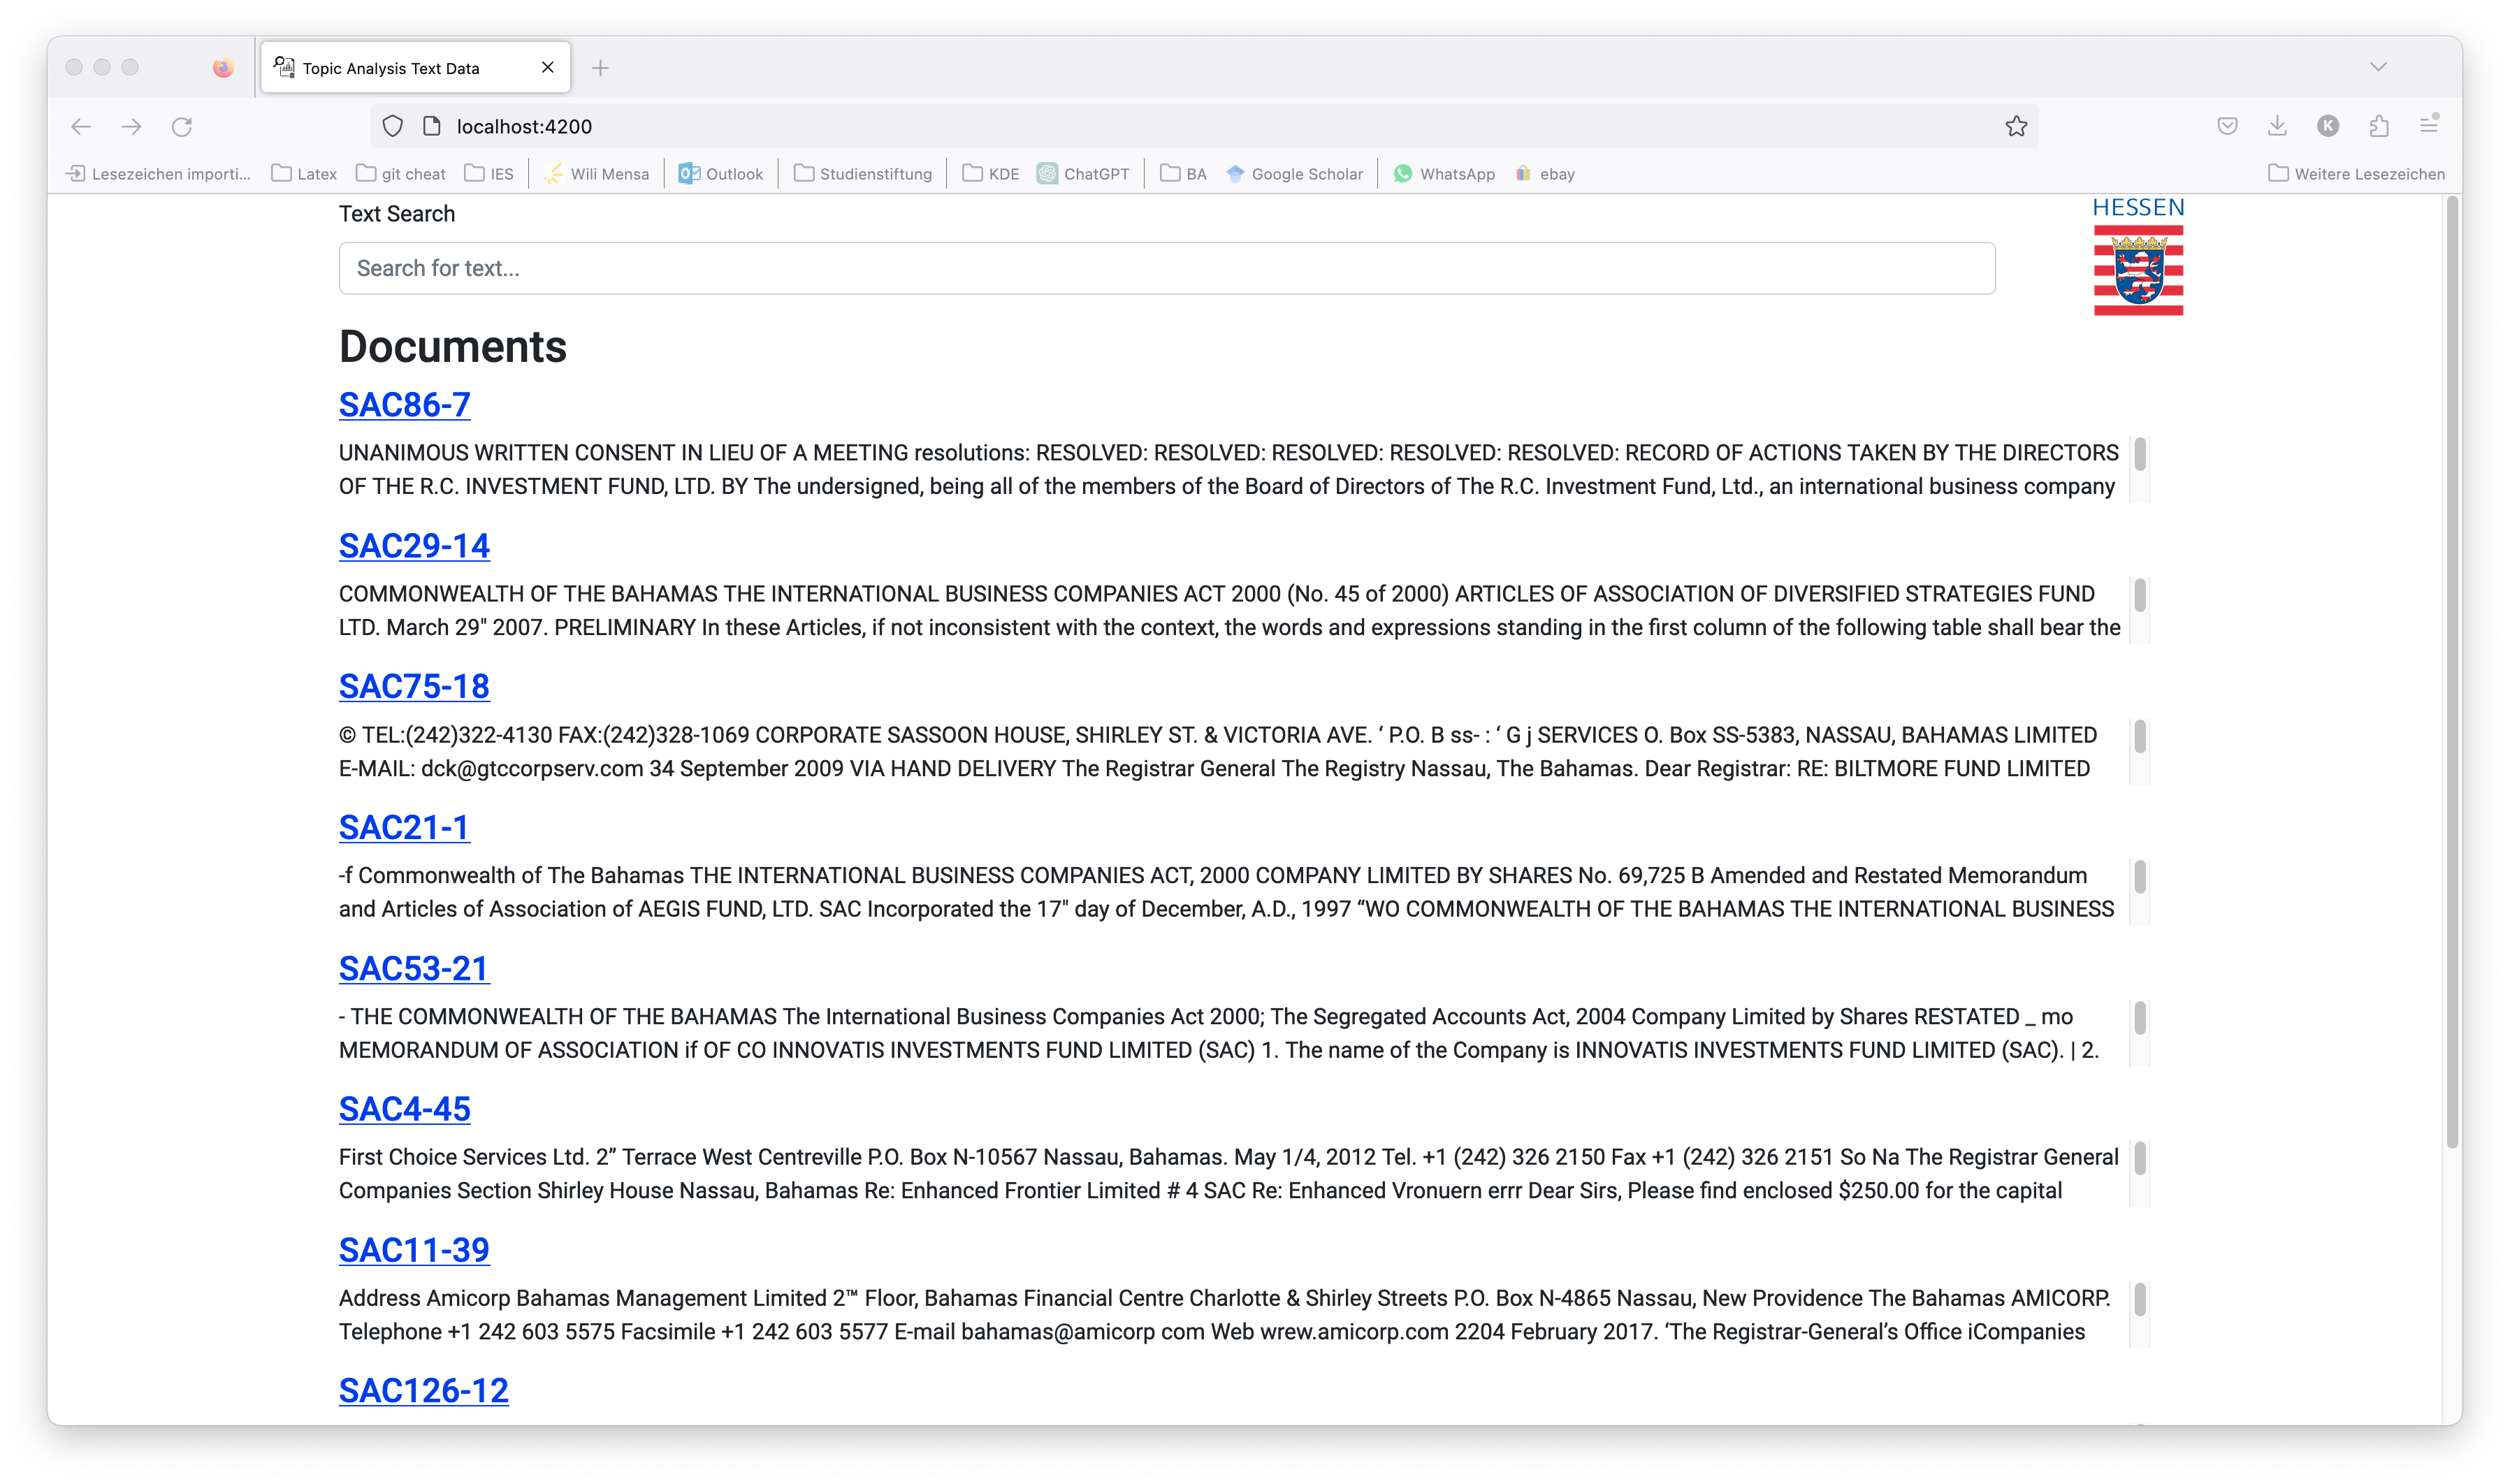
\includegraphics[width=0.7\textwidth]{images/UI/Home_component.png}
    \caption{Home component of the frontend.
    The search bar is used to enter the text query.
    The results of the query are displayed below the search bar.
    }
    \label{fig:home_comp}
\end{figure}


\begin{figure}[htp] % htp = hier (h), top (t), oder auf einer eigenen Seite (p).
    \centering
    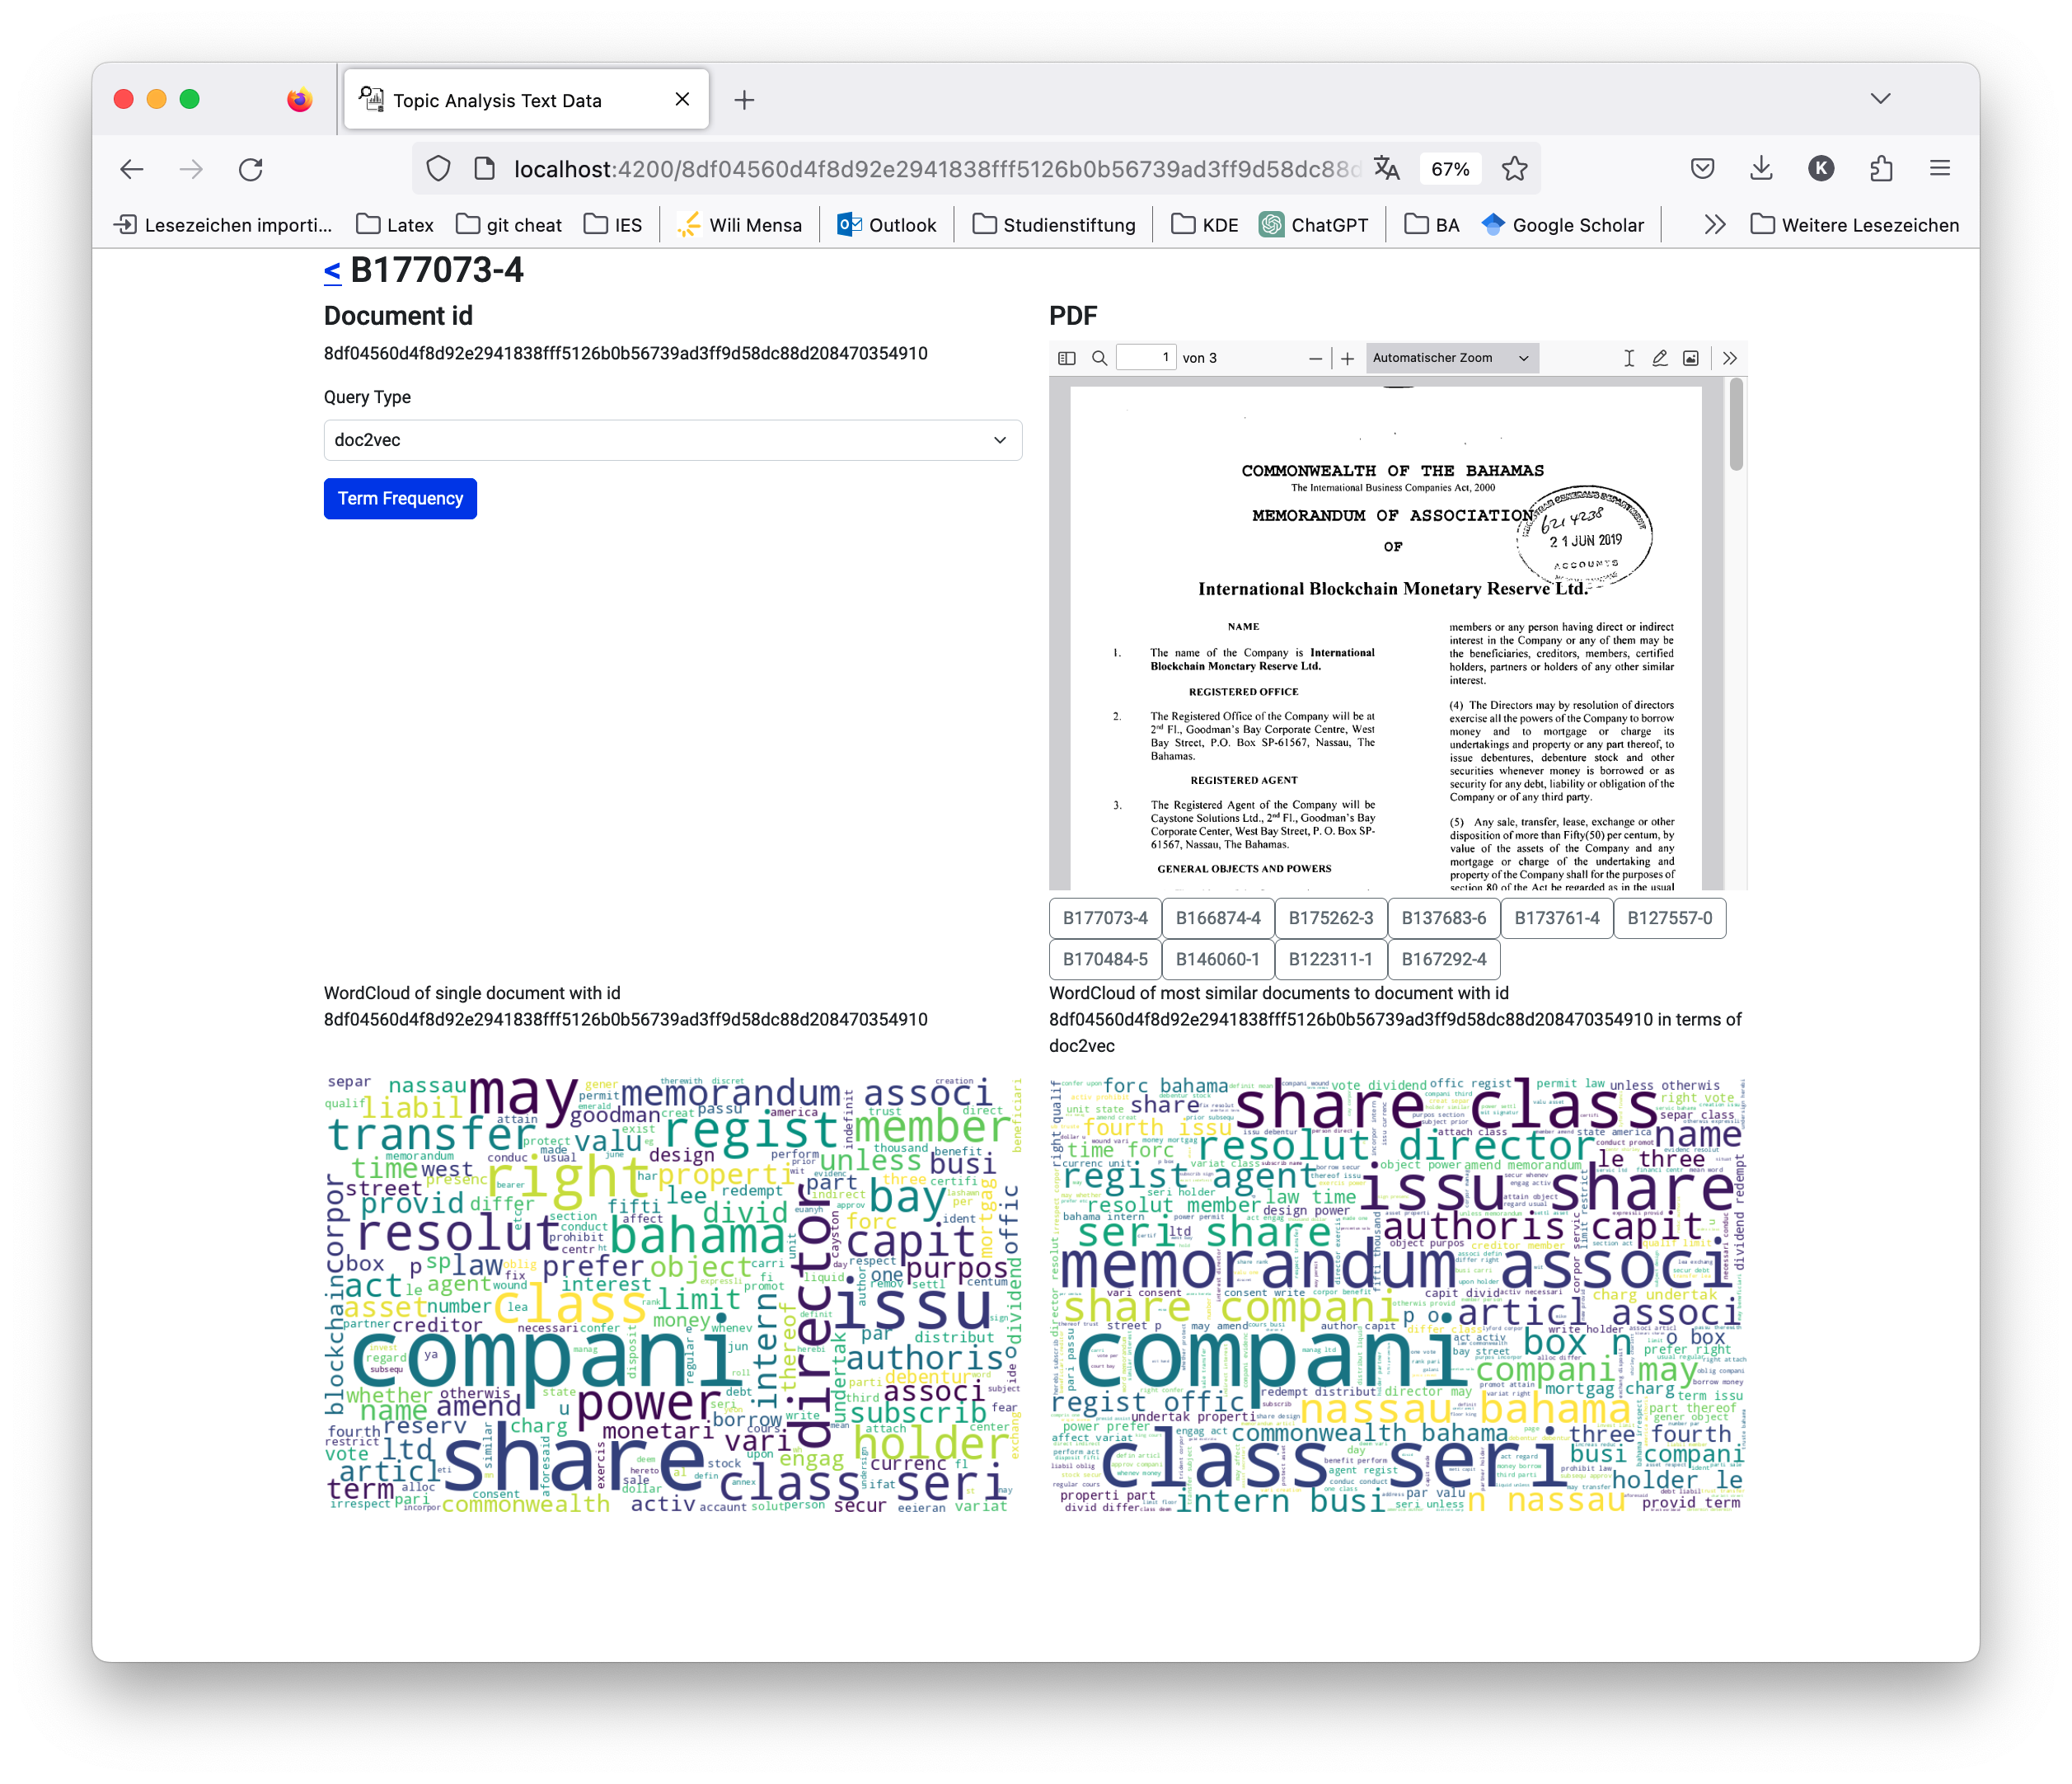
\includegraphics[width=0.7\textwidth]{images/UI/Home_detail.png}
    \caption{Detail component of the frontend.
    The chosen document is displayed, as well as its most similar documents in the database.
    WordClouds of the document and the most similar documents are displayed.
    }
    \label{fig:detail_comp}
\end{figure}


\begin{figure}[htp] % htp = hier (h), top (t), oder auf einer eigenen Seite (p).
    \centering
    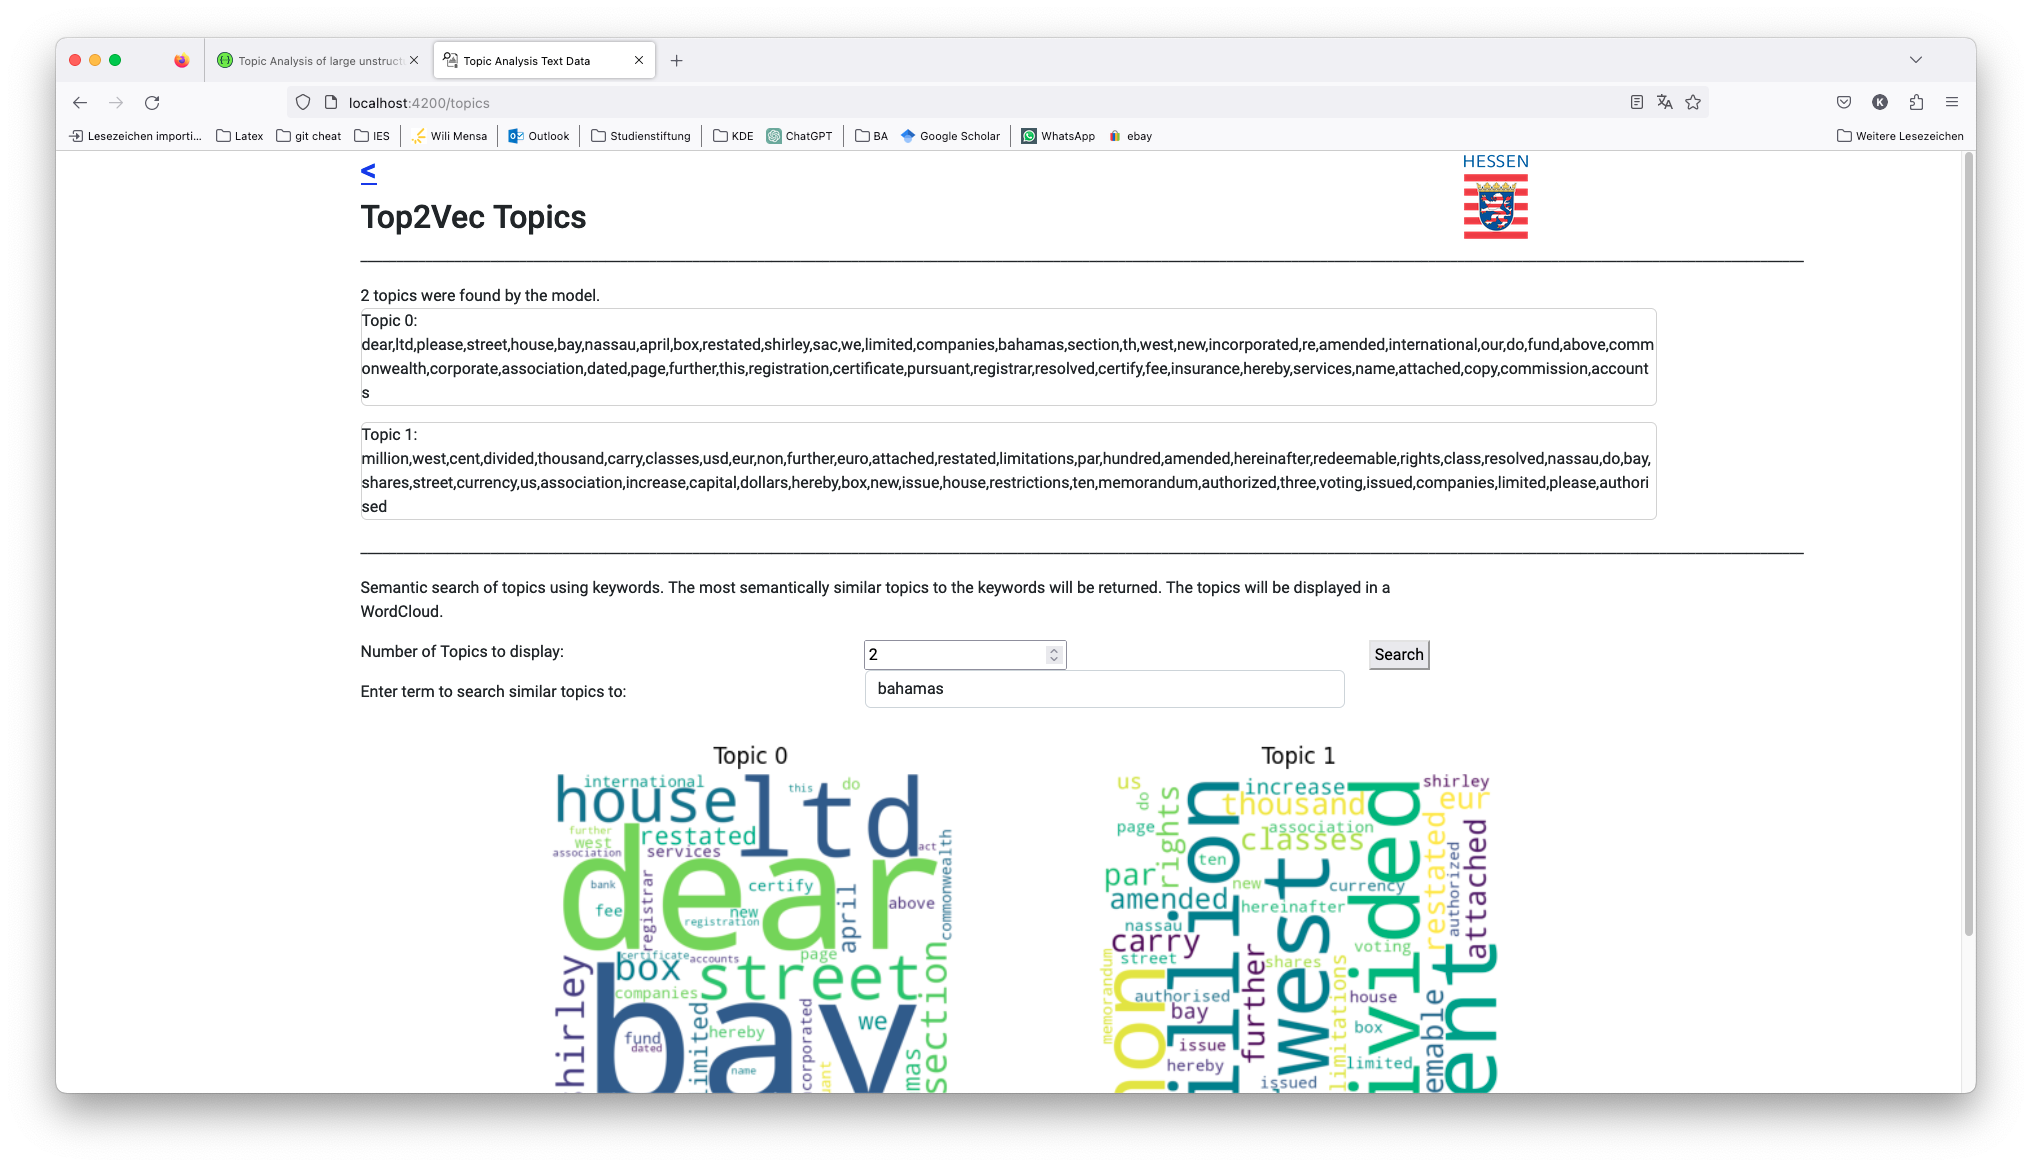
\includegraphics[width=0.7\textwidth]{images/UI/Top2Vec_Topics.png}
    \caption{Topic component of the frontend.
    }
    \label{fig:top2vec_topic_comp}
\end{figure}


To change between the components, the routes have to be defined.
The routes are defined in the \texttt{app-routing.module.ts} file, as shown in \autoref{lst:angular_routing}.

\begin{listing}[htp]
    \begin{minted}{typescript}
        const routes: Routes = [
            { path: ':id', component: DocumentDetailComponent},
            { path: '', component: HomeComponent},
          ];
    \end{minted}
    \caption{Definition of routes in \angular{} in the app-routing.module.ts.
    }
    \label{lst:angular_routing}
\end{listing}


\section{Trade-off between memory and query time}\label{sec:trade-off}

At the beginning of this thesis, it was unclear to what degree the tool, 
i. e. the database fields and query results should be precomputed.
A tool which is trained once offline is beneficial due to the amount of data.
Since \databaseName{} provides fast queries, it is sufficient to rely on real-time queries.

In the course of filling the database with information, 
one had to face obstacles not only regarding excessive memory usage but also long run times of methods.
Early on it became evident that one either had to reduce accuracy and details in order to achieve less memory or 
one had to settle for minutes to hours of calculations and bigger costs in terms of memory consumption.

Beforehand, it was not as clear which information, i. e. fields in the database, seemed worth the time and memory.
For instance, initially, the image of the first \ac{pdf} page of each document was saved alongside the other fields within the database.
After scaling the amount of data stored in the database to about 2900 documents, 
this approach caused severe issues in terms of memory usage.
Hence, this field is omitted.